\documentclass{beamer}
\usepackage[utf8]{inputenc}
\usepackage[ngerman]{babel}
\usepackage{graphicx}
\usepackage[export]{adjustbox}
\usepackage{listings}
\usetheme{AnnArbor}
\usecolortheme{beaver}
\setbeamertemplate{footline}%{infolines theme}
{
%\leavevmode%
%\hbox{
%\begin{beamercolorbox}[wd=.333333\paperwidth,ht=2.25ex,dp=1ex,center]{author in head/foot}%
%\usebeamerfont{author in head/foot}\insertshortauthor%~~(\insertshortinstitute)
%\end{beamercolorbox}%
%\begin{beamercolorbox}[wd=.333333\paperwidth,ht=2.25ex,dp=1ex,center]{title in head/foot}%
%\usebeamerfont{title in head/foot}\insertshorttitle
%\end{beamercolorbox}%
\begin{beamercolorbox}[wd=\paperwidth,ht=2.25ex,dp=1ex,right]{date in head/foot}%
\usebeamerfont{date in head/foot}\insertshortdate{}\hspace*{2em}
\insertframenumber{} / \inserttotalframenumber\hspace*{2ex}
\end{beamercolorbox}
%\vskip0pt%
}

\begin{document}
\title[]{Using Video Compression to Exploit Similarities in Biometric Databases
}
\author[]{Panteleimon Cheropoulos, Samy Dafir, Kevin Schörgnhofer}
\institute[]{Fachbereich Computerwissenschaften - Universität Salzburg}
\date[]{30. Juni 2017}

\frame{\titlepage}

\frame{\frametitle{Inhalt}\tableofcontents}

\section{Introduction}
\frame{\frametitle{Intro}
General incentive of this assignment: \\
\vspace{0.3cm}
"`Is it possible to effectively apply \textbf{video compression} for almost identical \textbf{pictures}?"' \\
\vspace{0.3cm}
$\rightarrow$ can we achieve \textit{better} results with video compression than with image compression?\\
$\rightarrow$ which codec is best suited for our purposes?\\
$\rightarrow$ how does the change of video codec parameters affect the results?\\
$\rightarrow$ how to determine the quality of the results?\\
}

\section{Setup}
\frame{\frametitle{Dataset}
The database consists of finger vein images of different fingers of different persons\\
\begin{itemize}
 \item 6 fingers per person, with 4 pictures per finger $\rightarrow$ 24 pictures per person
 \item 60 persons at all
 \item we worked with a subset of those
\end{itemize}
\begin{figure}[H]
 \centering
 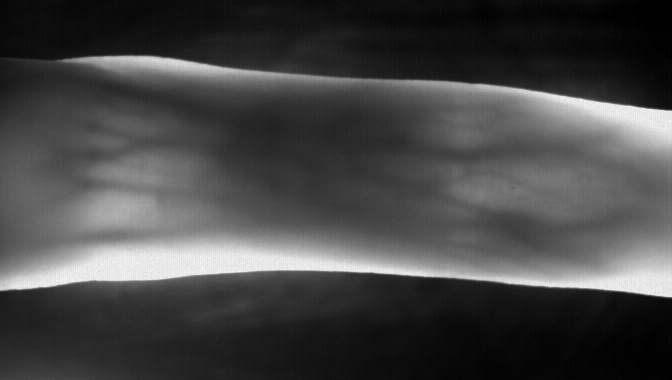
\includegraphics[width=0.5\textwidth]{graphics/fv_1_1.png}\hfill
 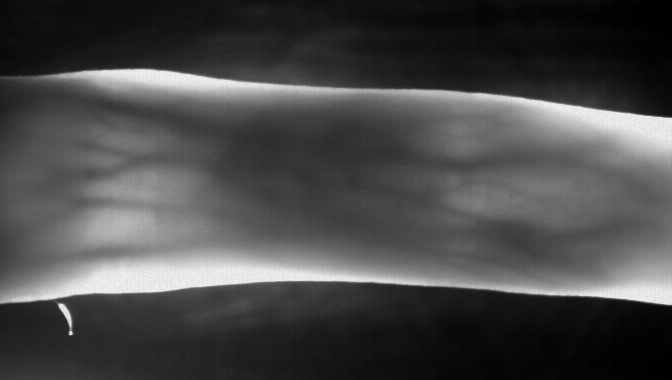
\includegraphics[width=0.5\textwidth]{graphics/fv_1_2.png}
\end{figure}
}

\subsection{Video Compression}
\frame{\frametitle{Video Compression}
\hspace{2cm}\huge Why video compression?
}

\frame{\frametitle{Video Compression}
	\underline{Why video compression?}
	\vspace{5mm}
	\begin{itemize}
		\item Very similar images
		\item Image compression only compresses individual images
		\item Video compression does 2 things:
		\begin{enumerate}
			\item Compresses images
			\item Exploits similarities between images
		\end{enumerate}
	\end{itemize}
}

\subsection{I,P,B-Frames}
\frame{\frametitle{I,P,B-Frames}
% http://www.tipterminal.de/pics/ipb_frames.gif
3 different types of pictures
\begin{itemize}
 \item I-Frame: Intra-coded picture
 \item P-Frame: Predictive-coded picture
 \item B-Frame: Bidirectional predictive-coded picture
\end{itemize}
\begin{figure}[H]
 \centering
 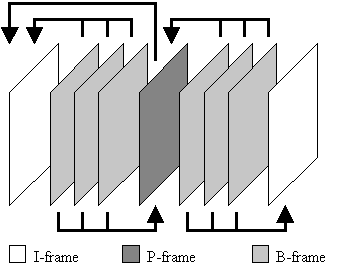
\includegraphics[width=0.5\textwidth]{graphics/ipb_frames.png}
\end{figure}
}

\subsection{Group Of Pictures}
\frame{\frametitle{Group Of Pictures}
\begin{itemize}
 \item usually defined with two numbers
 \begin{enumerate}
  \item defines distance of two I-Frames
  \item defines distance of two anchor frames (I or P)
 \end{enumerate}
 \item we used GOP to adapt the encoding to the database
 \begin{itemize}
  \item 24 pictures per person: use GOP 24 $\rightarrow$ 1 I-Frame per person
  \item 4 pictures per finger: use GOP 4 $\rightarrow$ 1 I-Frame per finger
 \end{itemize}
 \item P- and B-Frames allow higher compression $\rightarrow$ GOP affects the compression rate
\end{itemize}
}

\subsection{JPEG2000}
\frame{\frametitle{JPEG2000}
\begin{itemize}
 \item used as a baseline for comparison
 \item standard encoding settings, except number of layers
 \item ImageMagick (7.0.5-10) with integrated OpenJPEG library
 \begin{enumerate}
  \item encode pictures with jp2, with different compression rates
  \item determine quality of the pictures
  \item compare with pictures compressed with video codecs
 \end{enumerate}
\end{itemize}
}

\section{Quality Assessment}
\subsection{Matcher}
\frame{\frametitle{Matcher}

	\begin{itemize}
		\item Used as a "black box"
		\item Compares original and compressed images\\
		$\rightarrow$ Checks if matches found
		\item calculates different error metrics
		\item Target:\\
		\underline{Compare results of jpeg2000 and video compression}
	\end{itemize}
}

\frame{\frametitle{Error Metrics}

	\begin{itemize}
		\item FMR: False Match Rate
		\item FNMR: False Non Match Rate
		\item EER: Equal Error Rate
		\item Lower values are always better
	\end{itemize}

}

\frame{\frametitle{Error Metrics}
	\hspace{0.5cm}
	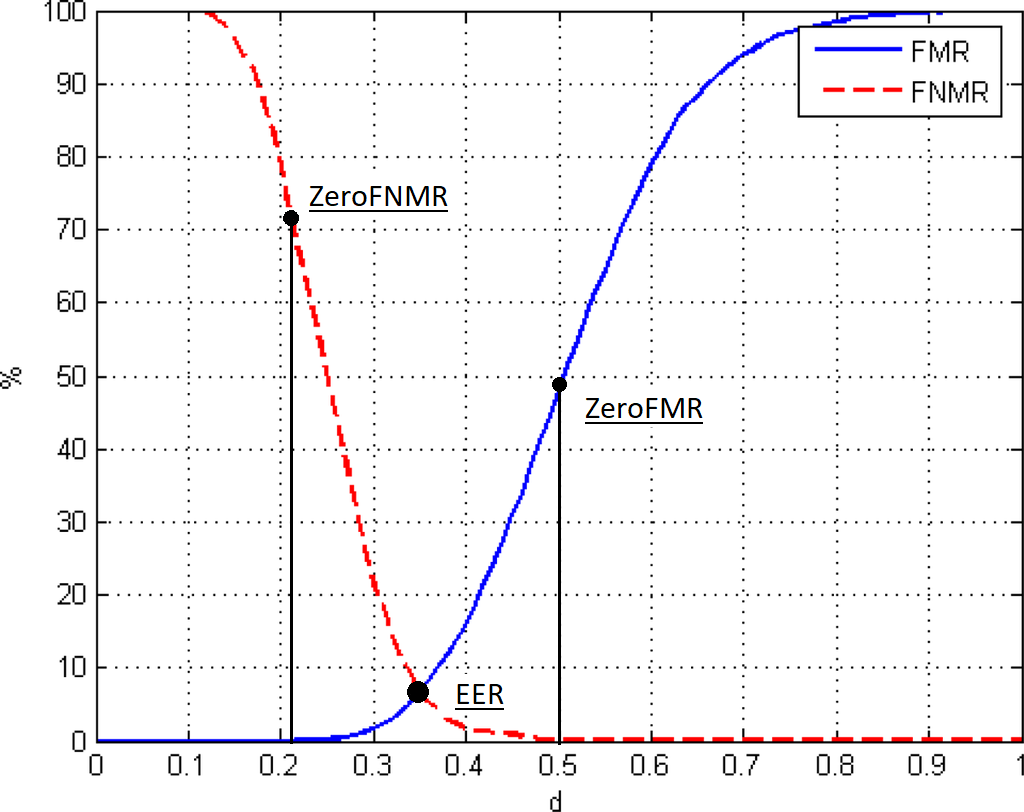
\includegraphics[width=8.5cm]{graphics/errors_modified.png}\\
	\tiny http://www.mdpi.com/sensors/sensors-11-09499/article\_deploy/html/images/sensors-11-09499f22-1024.png	
}

\section{CRF, Presets and Settings}
\frame{\frametitle{CRF}
\begin{itemize}
\item CRF value (Constant Rate Factor)
\begin{enumerate}
    \item The range of the quantizer scale is 0-51
    \item A lower value means better quality (0 for best quality, lossless)
    \item default value is 23
    \item A higher value means bad quality (51 for worst quality)
\end{enumerate}
\end{itemize}}

\frame{\frametitle{Presets}
\begin{itemize}
\item presets (they provide a certain encoding speed)
 \begin{enumerate}
   \item ultrafast , superfast , veryfast , faster , fast
   \item medium (default)
   \item slow, slower, veryslow, placebo
   \item we focused more to the slower presets (medium-veryslow)
 \end{enumerate}
 \end{itemize}}

 \frame{\frametitle{Settings}
 \begin{itemize}
\item what are the settings behind them?


\begin{center}
\begin{tabular}{ |c|c|c| }
 \hline
 medium & veryslow \\
 \hline
 \hline
 default & --b-adapt 2  \\
 \hline
 default & --partitions all  \\
 \hline
 default & --bframes 8  \\
 \hline
 default & --ref 16  \\
 \hline
\end{tabular}
\end{center}



\end{itemize}

}
 \frame{\frametitle{Settings}
  \begin{itemize}
    \item quick explanation of the settings :
    \begin{itemize}
        \item --b-adapt "Mod" : \\
        \begin{itemize}
        \item algorithm for the adaptive distribution of B-frames
        \item values : 0,1,2
        \end{itemize}
        \item --bframes "Max" : \\
        \begin{itemize}
        \item Defines how many B-frames can be positioned directly behind each other
        \item values are between 0 and 16 (3 is default)
        \end{itemize}

    \end{itemize}
  \end{itemize}
 }
\frame{\frametitle{Settings}
\begin{itemize}
\item --partitions "partitions" :\\
        \begin{itemize}
        \item partition size for macroblocks
        \end{itemize}
    \item --ref "frames" : \\
    \begin{itemize}
    \item amount of valid reference frames
    \end{itemize}

\end{itemize}
}

\frame{\frametitle{Settings (qscale mpeg4)}
\begin{itemize}
\item -qscale:v n
\item configure and select a video quality level
\item value for n : 1-31
\item 1 is the highest quality for largest filesize
\item 31 is the lowest quality for smalest filesize
\end{itemize}
}

\section{Implementation}
\subsection{Video Compression}
\frame{\frametitle{Video Compression}
	Setup:
	\begin{itemize}
		\item Used ffmpeg v.3.3.2 (latest version)
		\item Compressed 240 images
		\item Different crf values (0-50)
		\item Different qscale values for mpeg4 part 2
		\item Varying group of pictures (1, 4, 24)
		\item two presets (medium, veryslow)
	\end{itemize}


}

\frame{\frametitle{Video Compression}
	Repeat for each (crf, gop, preset) - combination
	\begin{enumerate}
		\item Compress images into single video
		\item get videosize (for compression rate)
		\item Decompress video $\rightarrow$ get images
		\item Put into folder named with settings
	\end{enumerate}
	Additional steps
	\begin{itemize}
		\item Collect image names $\rightarrow$ parameters for matcher
		\item rename decompressed videos
	\end{itemize}


}

\subsection{Matching}
\frame{\frametitle{Matching}
	\begin{itemize}
		\item Used matcher as "black box"
		\item Input:
		\begin{enumerate}
			\item original images
			\item compression output folders (crf, gop, preset)
		\end{enumerate}
		\item Match each output folder
		\item Retrieve error metrics
		\item Evaluate Error rate dependent on compression rate
	\end{itemize}

}


\section{Results}
\frame{\frametitle{Evaluation}
	\underline{Compression rate vs. matching errors}\\
	\begin{itemize}
		\item Group of pictures (1, 4, 24)
		\item Codecs (mpeg4 part 2, h.264, h.265)
		\item presets (medium, veryslow)
		\item Best result of jpeg2000 compression as baseline
	\end{itemize}
}

\frame{\frametitle{Comparing codecs}
	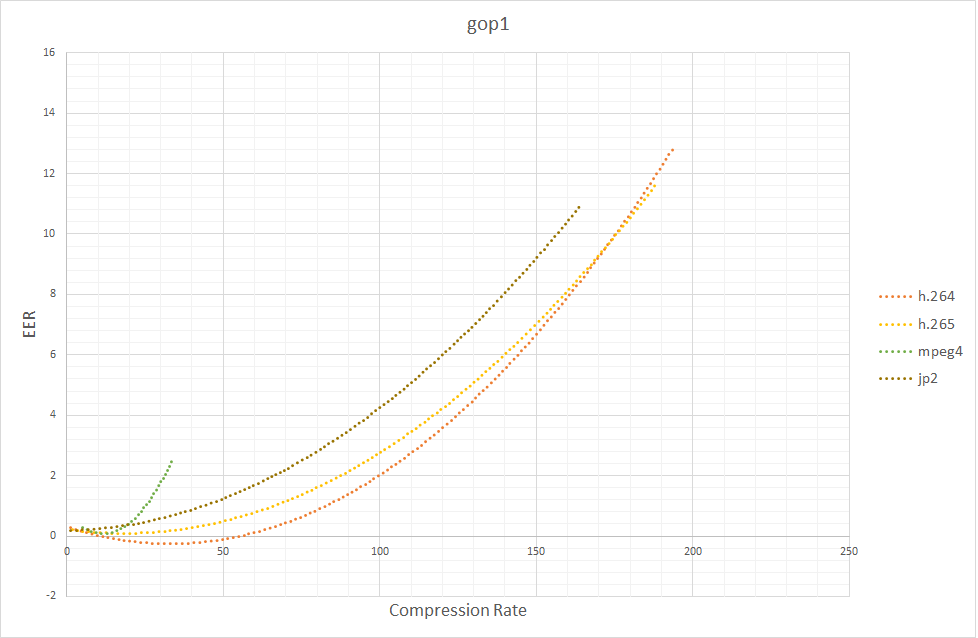
\includegraphics[width=11cm]{graphics/plot_7.png}
	
}

\frame{\frametitle{Comparing codecs}
	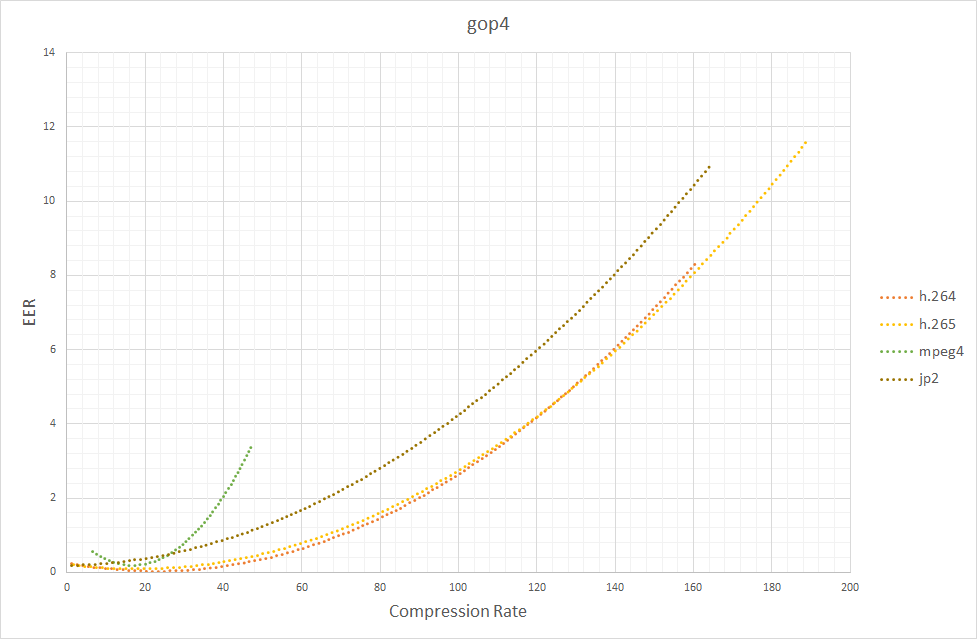
\includegraphics[width=11cm]{graphics/plot_8.png}	
	
}

\frame{\frametitle{Comparing codecs}
	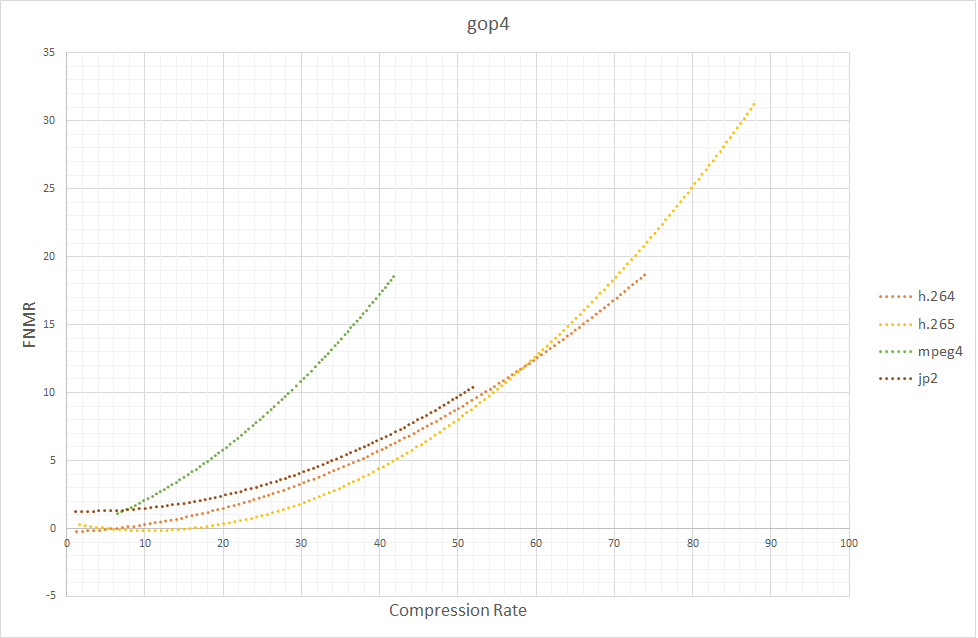
\includegraphics[width=11cm]{graphics/plot_11.png}	
	
}

\frame{\frametitle{Comparing codecs}
	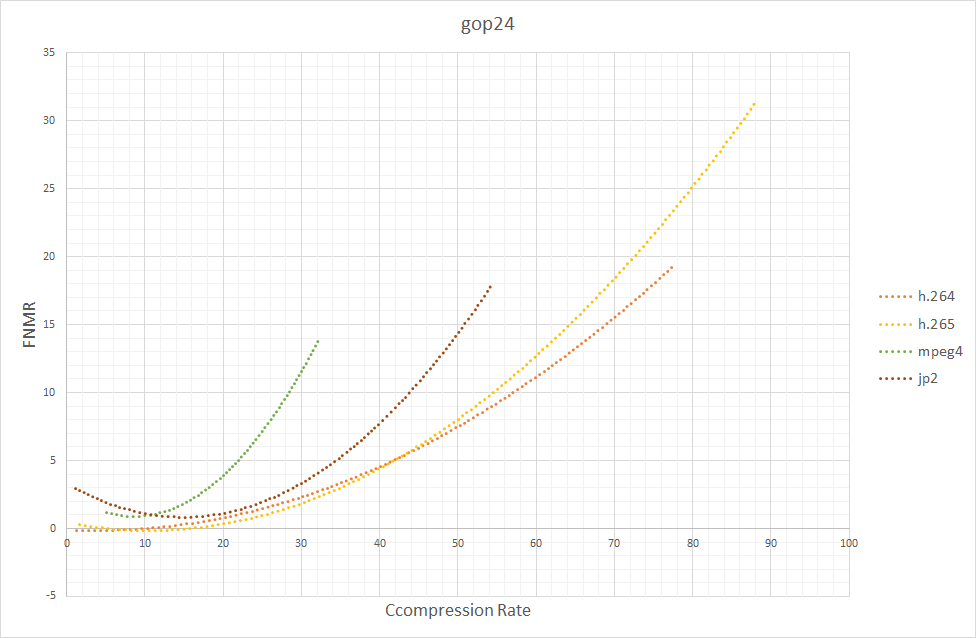
\includegraphics[width=11cm]{graphics/plot_12.png}	
	
}

\frame{\frametitle{Comparing group of pictures}
		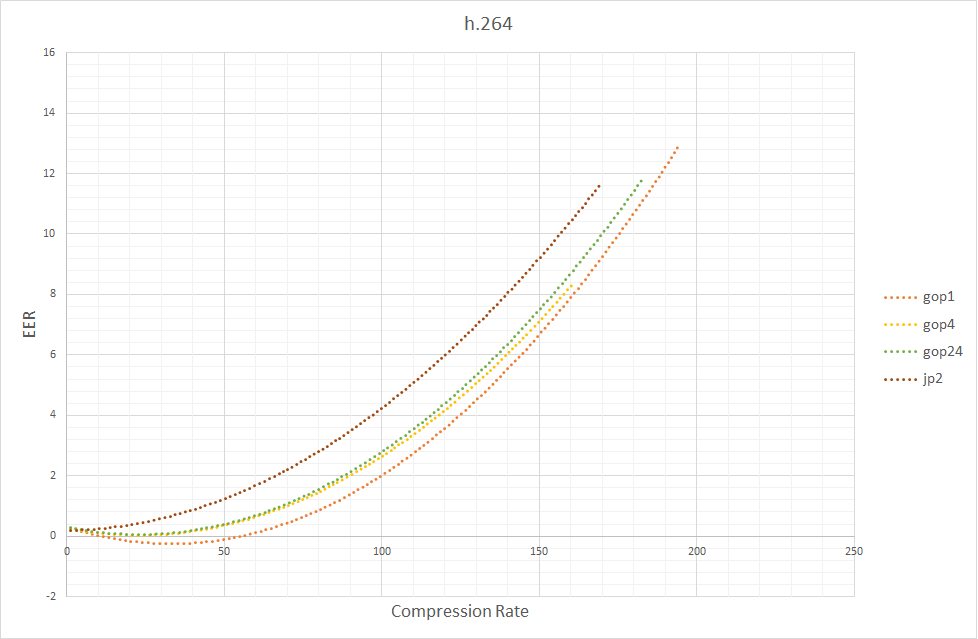
\includegraphics[width=11cm]{graphics/plot_1.png}
	
}

\frame{\frametitle{Comparing group of pictures}
		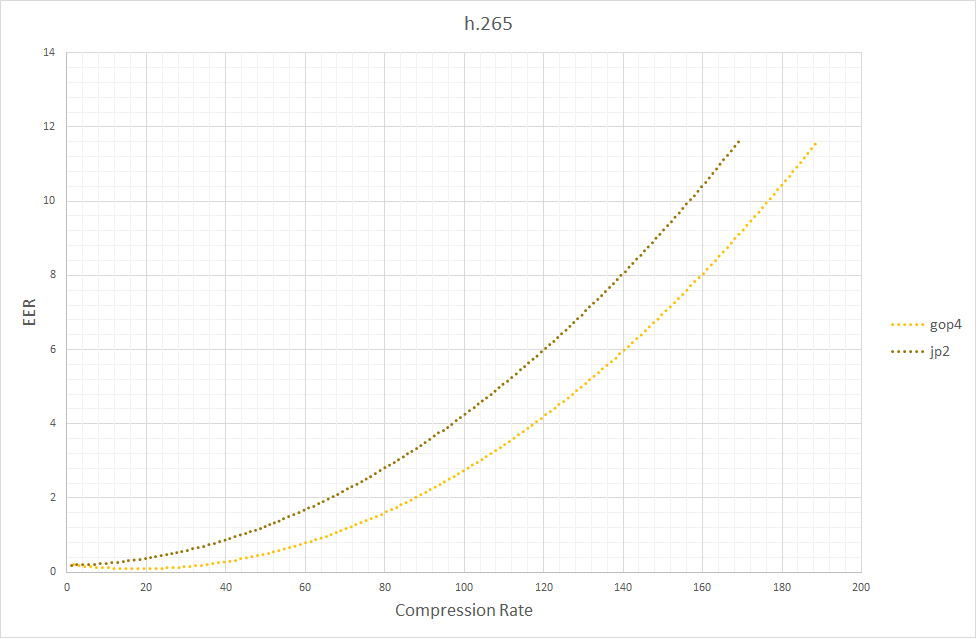
\includegraphics[width=11cm]{graphics/plot_2.png}
	
}

\frame{\frametitle{Comparing group of pictures}
		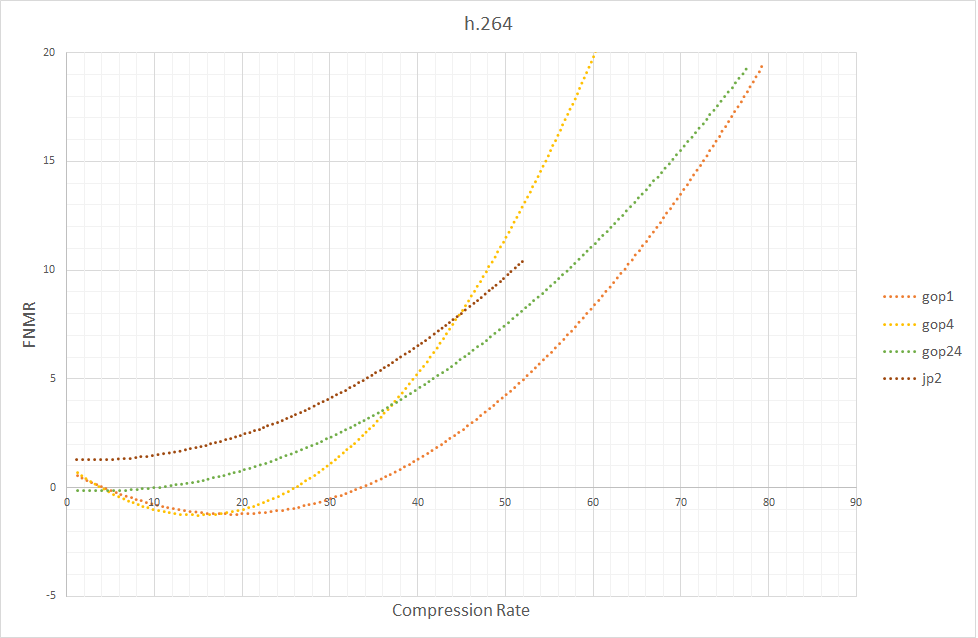
\includegraphics[width=11cm]{graphics/plot_4.png}
	
}

\frame{\frametitle{Comparing group of pictures}
		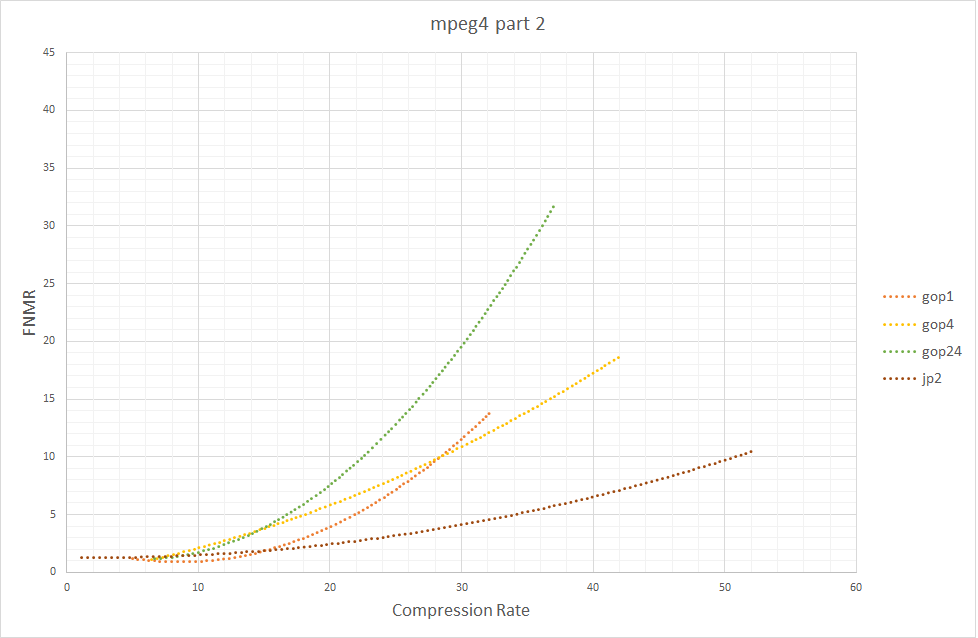
\includegraphics[width=11cm]{graphics/plot_6.png}
	
}

\frame{\frametitle{Comparing presets}
	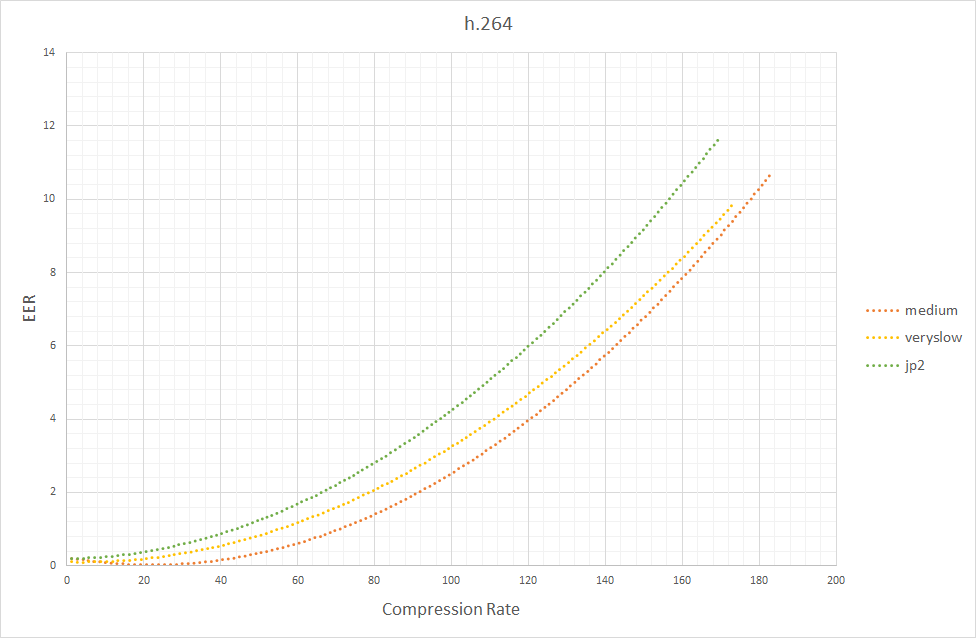
\includegraphics[width=11cm]{graphics/plot_13.png}
	
}

\frame{\frametitle{Comparing presets}
	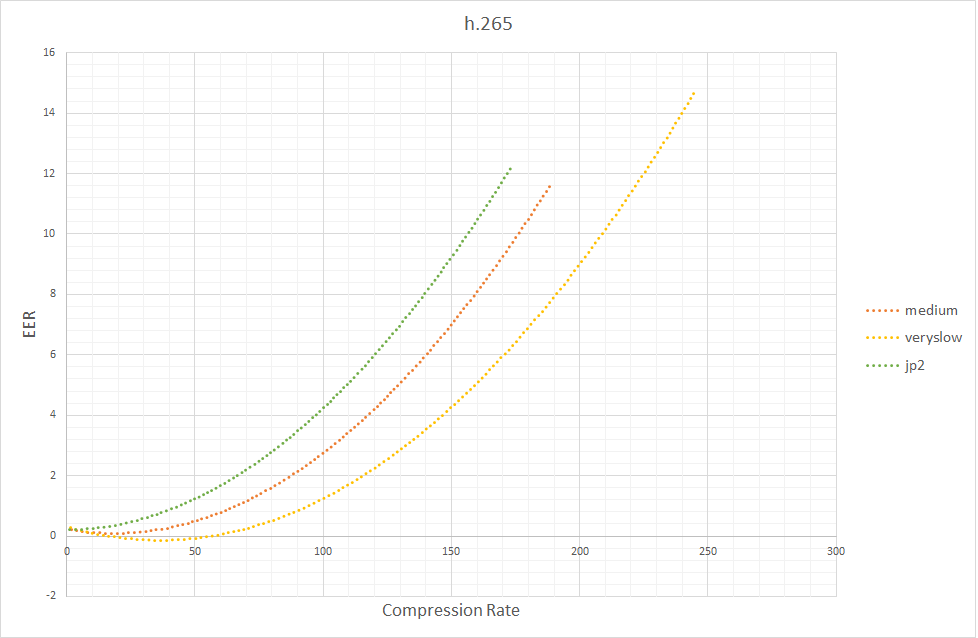
\includegraphics[width=11cm]{graphics/plot_14.png}
	
}

\frame{\frametitle{Comparing presets}
	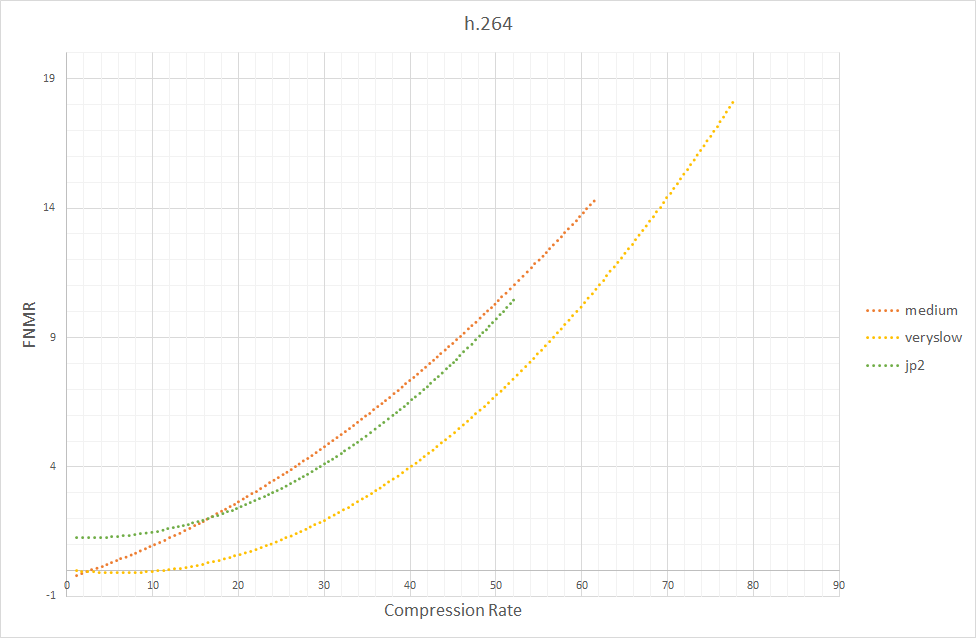
\includegraphics[width=11cm]{graphics/plot_15.png}
	
}


\frame{\frametitle{Conclusion}
	\underline{Best Results:}
	\vspace{5mm}
	\begin{itemize}
		\item GOP 1
		\item h.264 or h.265
		\item veryslow
	\end{itemize}
	\vspace{5mm}
	40\% higher compression at same EER (h.265 veryslow)\\
	30\% higher compression at same FNMR (h.264 veryslow)
	
	
	
}

\frame{
	\vspace{5mm}
	\centering
	\huge Thank you for your attention!
}

\end{document}


























